% ========== Choix techniques ===========
\section{Choix techniques}

  \subsection{Logique métier}
    \begin{frame}
      \frametitle{Choix techniques}
      \begin{itemize}
        \item Langage de programmation: \textbf{Java} \vspace{1cm}
        \item Communication client-serveur: \textbf{RMI}
        \begin{itemize}
          \item Orienté objet
          \item Gestion des exceptions
        \end{itemize}
      \end{itemize}
    \end{frame}

  \subsection{Graphisme}
    \begin{frame}
      \frametitle{Choix techniques}
      \begin{itemize}
        \item Interface graphique: \textbf{Slick2D}
      \end{itemize}
      \begin{center}
        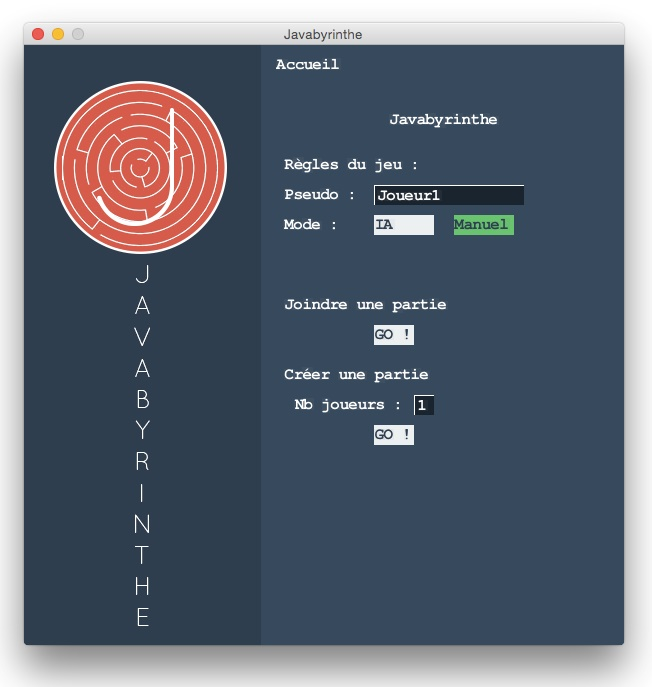
\includegraphics[scale=0.4]{image/menuJavabyrinthe.jpg}
      \end{center}
    \end{frame}
